\chapter{Metodología}

\subsection{Fundamentación}
Para el desarrollo de los sistemas que conforman el macro-proyecto \textbf{“Gestión de Calidad”}, incluyendo el módulo de \textbf{gestión de evidencias} y el módulo de \textbf{gestión de tiempos de jornada}, se adoptó la metodología ágil \textbf{Scrum}.  

Esta decisión se basa en la necesidad de gestionar un proyecto modular y complejo, con requisitos que evolucionan en función de los procesos de acreditación universitaria (SINAES) y de la dinámica institucional.  

Las principales razones de su selección incluyen:
\begin{itemize}
    \item \textbf{Entregas incrementales}: se realizan entregas funcionales frecuentes a los diferentes stakeholders (Comité de Calidad SINAES, administración, docentes), permitiendo retroalimentación continua.
    \item \textbf{Flexibilidad y adaptabilidad}: Scrum facilita la incorporación de cambios en los criterios de acreditación y en las necesidades de los usuarios sin afectar la planificación global.
    \item \textbf{Alineación con el cronograma académico}: la iteración por sprints se ajusta a los semestres académicos y a los avances parciales solicitados en el curso.
    \item \textbf{Modularidad}: la arquitectura de los módulos permite construir bases funcionales mínimas y agregar nuevas características progresivamente.
\end{itemize}

\subsection{Referencia al WBS}
El marco metodológico se complementa con la \textbf{Estructura de Desglose del Trabajo (WBS)}, que organiza los entregables y actividades principales del proyecto en fases y módulos. El WBS fue elaborado en una herramienta formal (\emph{WBS Schedule Pro}), conforme a la observación docente, y sirve de guía para la planificación de sprints y la asignación de responsabilidades.

La Figura~\ref{fig:wbs} muestra la estructura jerárquica del proyecto y su correspondencia con los artefactos de Scrum:
\begin{itemize}
  \item \textbf{Nivel 1 (Proyecto):} alcance global del macro-proyecto \emph{Gestión de Calidad}.
  \item \textbf{Nivel 2 (Módulos/Fases):} Evidencias SINAES, Tiempos de Jornada, Integración/QA, Documentación/Estándares, Despliegue/Cierre.
  \item \textbf{Nivel 3 (Entregables):} análisis, diseño UI/UX, implementación (CRUDs, reportes), pruebas, documentación.
  \item \textbf{Nivel 4 (Paquetes de trabajo):} tareas planificables en sprints (vinculadas al \emph{Sprint Backlog}).
\end{itemize}

\begin{figure}[H]
  \centering
  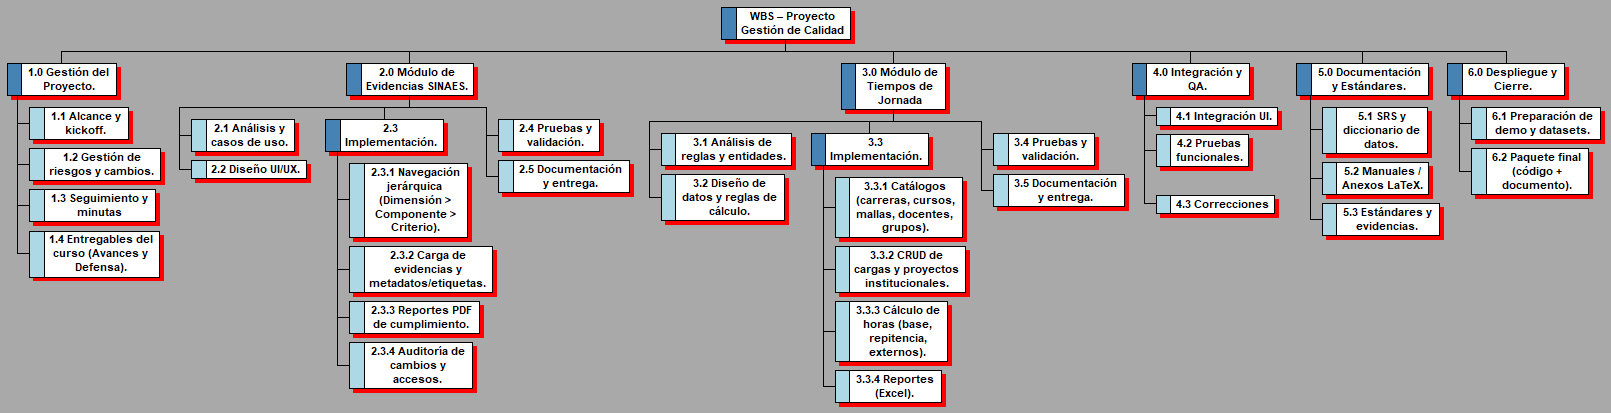
\includegraphics[width=\textwidth]{figs/wbs_chart.png}
  \caption{Estructura de Desglose del Trabajo (WBS) del proyecto.}
  \label{fig:wbs}
\end{figure}

Para referencia en alta resolución, el diagrama completo se incluye también en el \hyperref[anexo:wbs]{Anexo 7: WBS (Estructura de Desglose de Trabajo)}.

\subsection{Aplicación al proyecto}
La adaptación de Scrum al macro-proyecto \textbf{Gestión de Calidad} se realizó con los siguientes lineamientos:

\begin{itemize}
    \item \textbf{Roles:}
    \begin{itemize}
        \item \textbf{Product Owner (PO):} Comité de Calidad de la UNA y profesores responsables, quienes priorizan y validan entregables.
        \item \textbf{Scrum Master:} rol asumido de forma rotativa entre los estudiantes, garantizando disciplina metodológica.
        \item \textbf{Equipo de Desarrollo:} integrado por los 2 estudiantes responsables de la construcción de los módulos.
    \end{itemize}

    \item \textbf{Eventos:}
    \begin{itemize}
        \item \textbf{Sprint Planning:} definición de objetivos y tareas cada dos semanas.
        \item \textbf{Daily Scrum:} reuniones virtuales de 15 minutos para seguimiento y bloqueos.
        \item \textbf{Sprint Review:} demostración de los incrementos funcionales al PO al cierre de cada sprint.
        \item \textbf{Sprint Retrospective:} análisis del proceso y propuestas de mejora.
    \end{itemize}

    \item \textbf{Artefactos:}
    \begin{itemize}
        \item \textbf{Product Backlog:} listado priorizado de requerimientos funcionales (RF-01 al RF-17).
        \item \textbf{Sprint Backlog:} conjunto de tareas planificadas en cada sprint.
        \item \textbf{Incremento:} entregables funcionales validados al cierre de la iteración.
    \end{itemize}

    \item \textbf{Ajustes específicos:}
    \begin{itemize}
        \item \textbf{Duración de sprint:} 2 semanas, alineadas con los avances del curso.
        \item \textbf{Entregas formales:} vinculadas a los Avances 1, 2, 3 y a la Defensa Final.
        \item \textbf{Herramientas:} GitHub Projects para gestión de backlog, GitHub Actions para CI/CD y Google Drive para almacenamiento y evidencias.
    \end{itemize}
\end{itemize}

De esta forma, Scrum se implementa como una metodología realista y adaptable, con foco en entregas funcionales que aseguran el cumplimiento de los criterios académicos y de acreditación.
